\section{Parameter calibration and pseudo-forcing attribution against MODIS LST}
\label{app:modis-calibration}

This appendix documents the gradient-based experiments that precede the
surface-layer closure of Sect.~\ref{sec:structural-slab}: an
observation-space information analysis, an observing-system simulation, a
parameter calibration against real MODIS observations, a pseudo-forcing
attribution, and the forward timescale-asymmetry sweep that brackets the
closure's two relaxation times. Their role is diagnostic rather than
corrective: the table-scale calibration removes little of the bias in either
window, and the pseudo-forcing profile, though seasonally robust under the
anchored evaluation, is an additive forcing adjustment with no process form.
Together they
establish the two facts the closure builds on: the reverse-mode inversion
machinery is sound, and the daytime cold bias is structural, with a specific
diurnal shape that no admissible parameter correction supplies;
Sect.~\ref{sec:bias-attribution} states this attribution in the main text. All experiments use the spun-up initial
state of Sect.~\ref{sec:modis-evaluation}, ten autumn--winter calibration days
and ten held-out spring--summer days, the strict-QC day and night MODIS
channels, and $\cos\phi$ area weighting; the closure of
Sect.~\ref{sec:structural-slab} reuses the same protocol.

\subsection{Observation-space parameter identifiability}
\label{sec:modis-identifiability}

The existence of a reverse-mode derivative does not imply that a parameter
can be inferred from a given observation set. We therefore used the MODIS LST
operator of Sect.~\ref{sec:modis-evaluation} to diagnose the local
information content before attempting parameter optimization. Four seasonally
matched one-day windows were initialized from the corresponding annual state
archive, each after a 24~h unperturbed closure adjustment, with the model LST
sampled at the cell-specific MODIS view times under the strict QC mask and
$\cos\phi$ area weights. The control vector comprised three dimensionless,
logarithmic scaling directions applied to the vegetation lookup tables
(leaf-area index, minimum stomatal resistance, momentum roughness length).
If $\boldsymbol{r}$ is the area-weighted, QC-filtered LST residual vector
and $\boldsymbol{J}=\partial\boldsymbol{r}/\partial\log\boldsymbol{s}$, the
local Gauss--Newton information matrix is
$\boldsymbol{F}=\boldsymbol{J}^{\mathsf{T}}\boldsymbol{J}$, estimated with 16
fixed-seed Rademacher reverse-mode projections.

The information content was evaluated separately for the spring--summer and
the autumn--winter windows. The spring--summer
information eigenvalues were $1.57\times10^{7}$, $4.41\times10^{2}$, and
$53.0$, giving a condition number of $2.96\times10^{5}$; the autumn--winter
eigenvalues were 54.8, 5.65, and 0.823, with a condition number of 67. The
strong spring--summer collinearity is also visible in
Fig.~\ref{fig:modis-identifiability}: the normalized
leaf-area--stomatal-resistance information correlation is $-0.99$,
whereas the autumn--winter correlations are much smaller in magnitude. The
same differentiable model is
thus locally ill-conditioned in one season and substantially better
constrained in another, a property of the physics and observing pattern,
not of the optimizer, and it dictates the design of the calibration.

\begin{figure}[t]
\centering
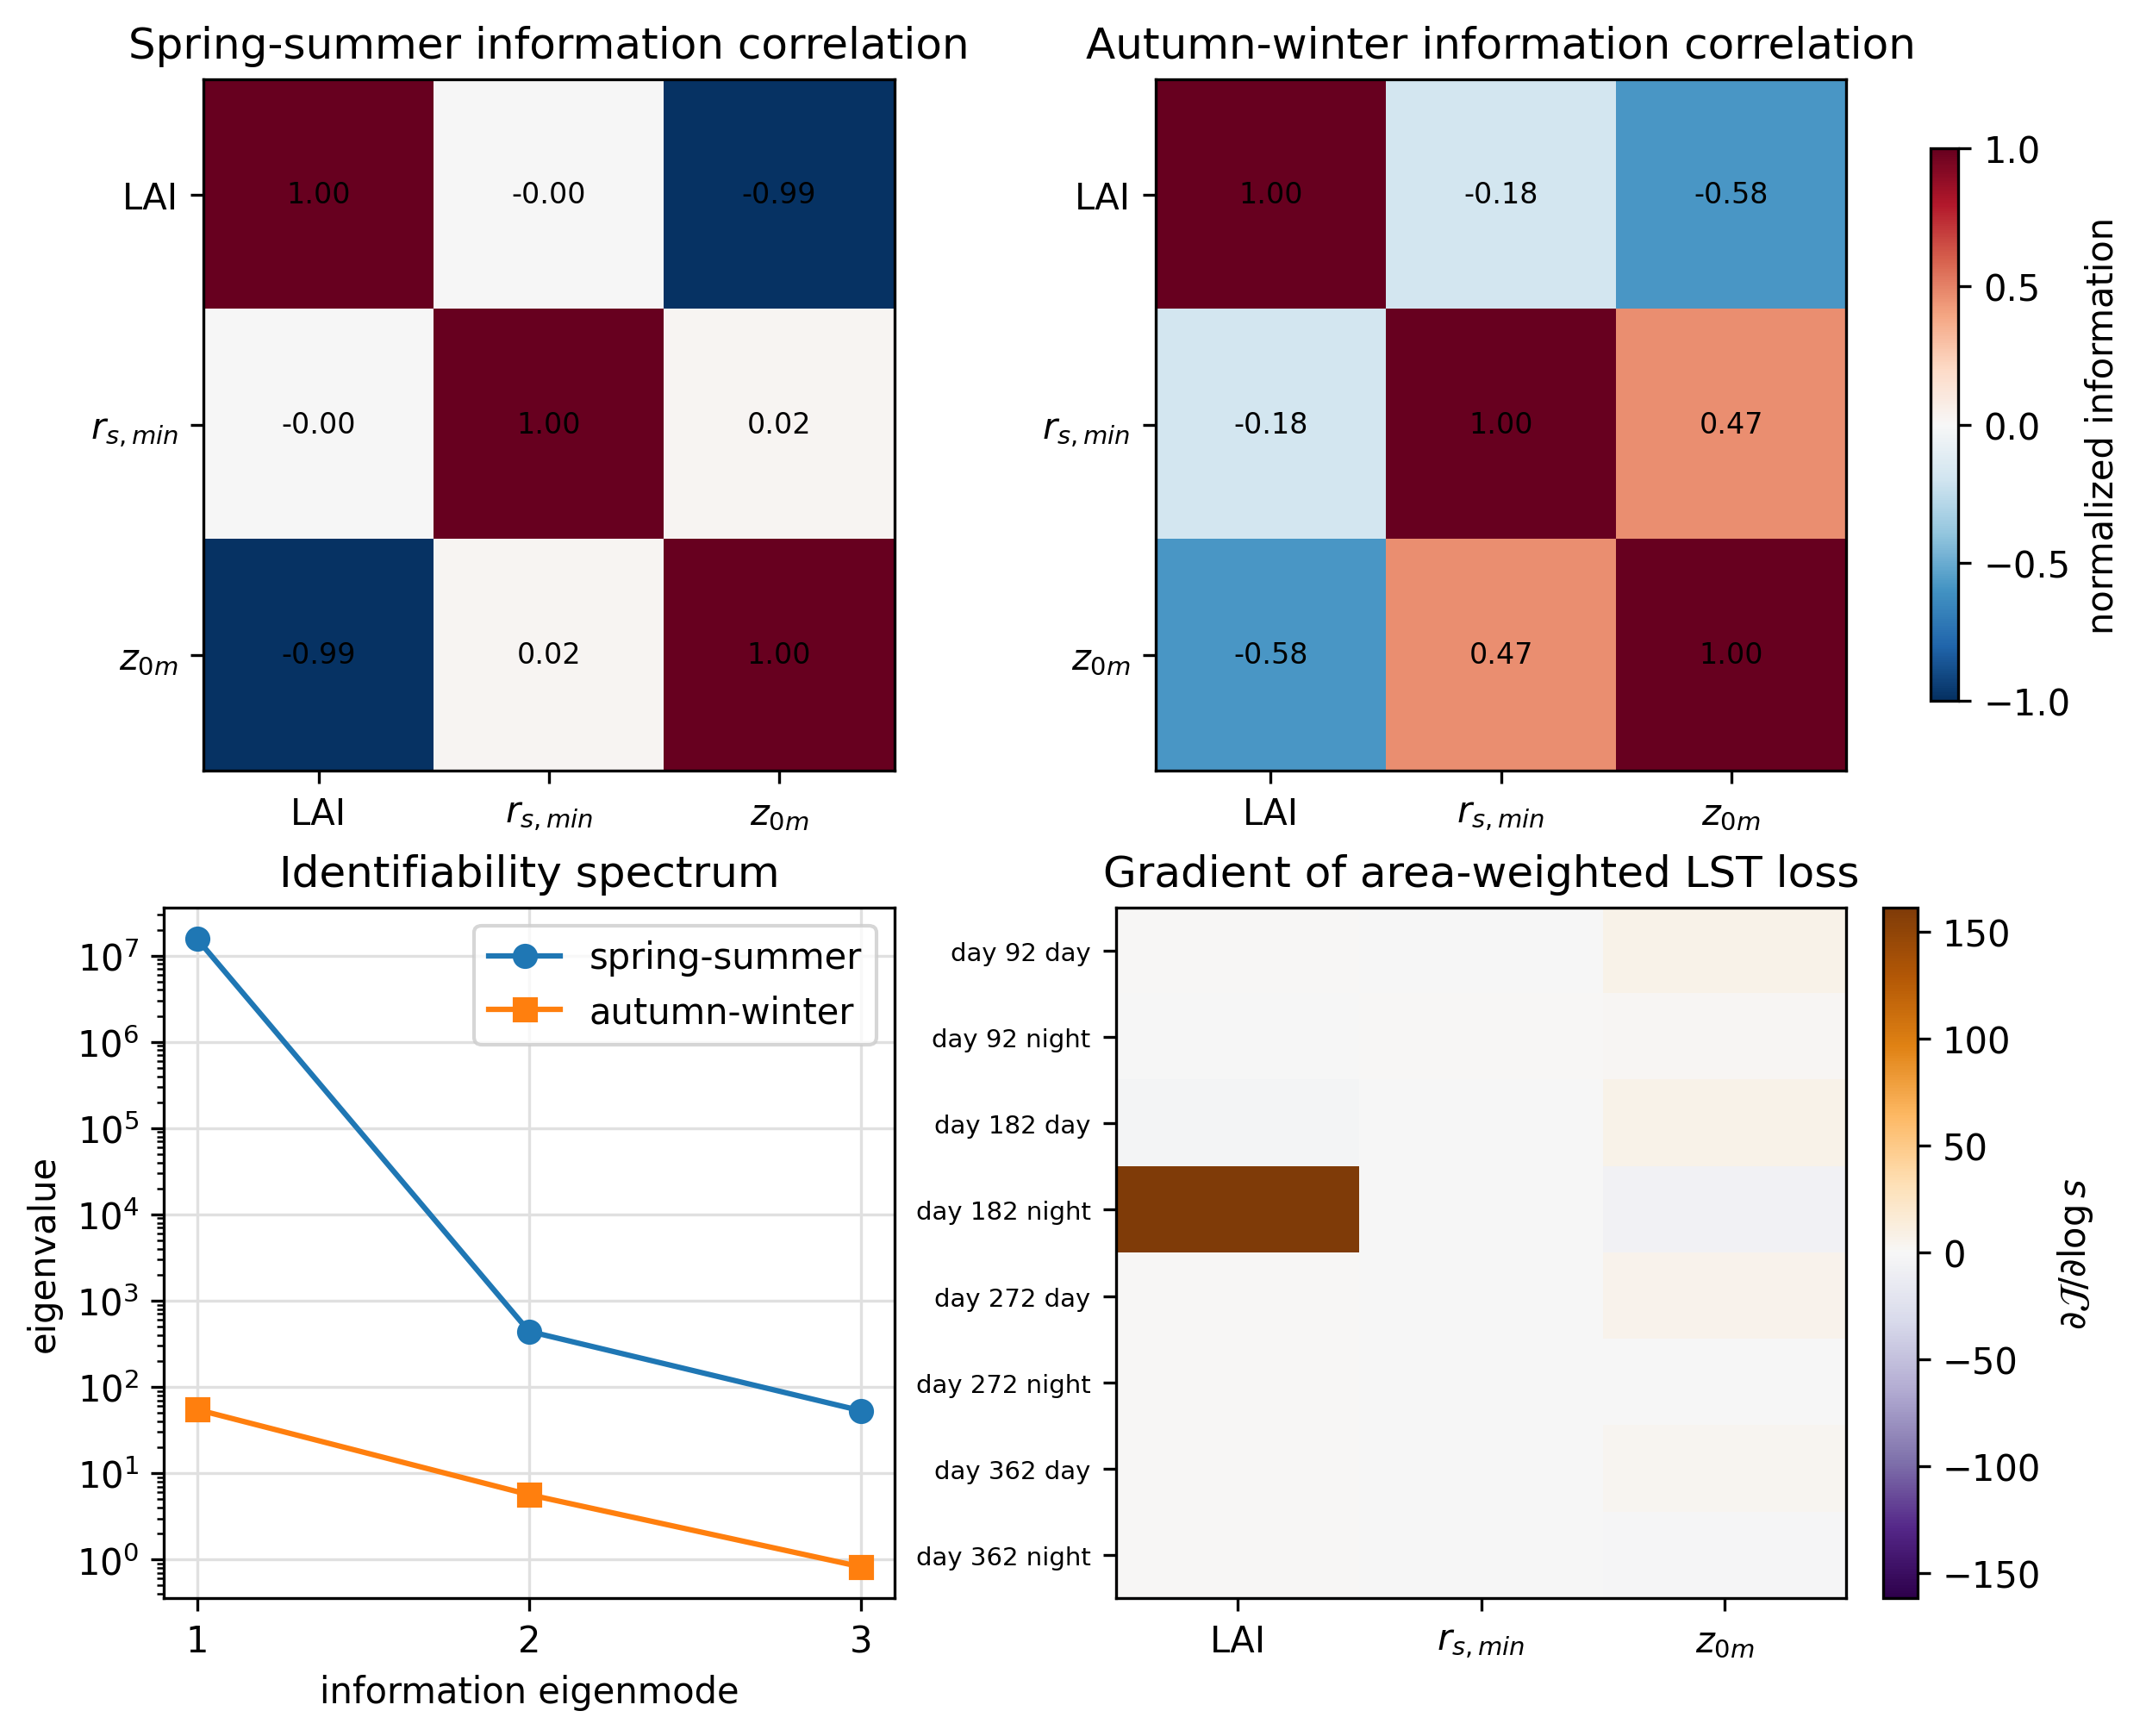
\includegraphics[width=\linewidth]{figures/modis_parameter_identifiability.png}
\caption{MODIS LST observation-space identifiability of three logarithmic
vegetation scaling controls. Upper panels show normalized information
correlations for the spring--summer and the
autumn--winter windows. Lower left gives the corresponding
information eigenvalues; lower right gives the seasonal LST-loss gradients.
The matrices are area-weighted and computed from strict MODIS QC samples.}
\label{fig:modis-identifiability}
\end{figure}

\subsection{Conditioned-window calibration against MODIS LST}
\label{sec:modis-calibration}

Guided by the identifiability diagnostic, the seasonal split is inverted:
multiplicative parameter-table scales are fitted in ten well-conditioned
autumn--winter windows and evaluated on ten held-out spring--summer windows
that never enter the loss (2018; days of year 271, 281, $\dots$, 361 and
91, 101, $\dots$, 181, respectively, the same window set as the closure
calibration of Sect.~\ref{sec:structural-slab}). Each window restores the
land state from the daily archive of the autonomous, unclosed 2018
integration at the previous day boundary, advances 48 physics steps
without gradients so that fast variables re-equilibrate, and then integrates
a further 48 steps with the radiative skin temperature sampled at each
column's strict-QC MODIS overpass time, separately for the day and night
passes. Training uses every fifth CMFD column (19{,}542 of 97{,}709;
column-independent offline dynamics are unchanged), and every reported
verification statistic uses the full domain: 73{,}700 daytime and
15{,}491 nighttime calibration samples, and 131{,}030 and 62{,}077 held-out
samples.

The control vector contains eight multiplicative table scales: the
leaf-area-index, minimum-stomatal-resistance, and roughness-length vegetation
tables, each split between the domain's high- and low-vegetation classes, a
joint scale on the dry and saturated soil thermal-conductivity end-members,
and a scale on the dry-soil heat-capacity table. Writing $s_j$ for the
logarithm of scale $j$, the affected table entries are set to
$\bar{T}_{j,e}\,e^{s_j}$ on the class mask, and the loss aggregates the
area-weighted mean-squared LST residual over all strict-QC samples of the ten
calibration windows,
\begin{equation}
  \mathcal{J}(\boldsymbol{s}) = \sum_{d\in\mathcal{C}}
    \sum_{p\in\{\mathrm{day},\,\mathrm{night}\}}
    \frac{\sum_i \cos\phi_i\,
      \left[T^{\mathrm{mod}}_i(t_i;\boldsymbol{s})-T^{\mathrm{obs}}_i\right]^2}
         {\sum_i \cos\phi_i}.
\label{eq:calib-loss}
\end{equation}
One reverse pass through the 48 gradient steps differentiates the loss with
respect to every table element, from which the scale derivatives follow by
the chain rule, so a single forward--backward calculation per window trains
all eight controls simultaneously. The scales are updated with Adam
(learning rate 0.02) and bounded in $[1/2,2]$, and the state is freshly
restored from the archive every iteration, so no parameter-induced drift
accumulates.

A no-gradient leverage probe on the first calibration day fixes the control
selection: the three high-vegetation scales change the loss by exactly zero
on this snow-free day (the structural zero-gradient case of
Sect.~\ref{sec:gradient-interpretation}), while the low-vegetation roughness
scale dominates ($|\Delta\mathcal{J}|\approx0.97$ per $\pm10\%$, an order of
magnitude more than any other active control), which motivates splitting the
vegetation tables by class. In an observing-system simulation with the real
operator, overpass times, and QC masks, synthetic observations from known
truths (roughness scale $0.70$, soil heat-capacity scale $1.40$) plus 1~K
noise, the documented MODIS accuracy, the same loop
recovers the truths to within 0.3--1.1\,\% (roughness recovered to 0.692,
heat capacity to 1.404), drives the training loss to its
analytic noise floor, and transfers to the held-out days; the two
unperturbed but collinear controls drift to compensating values, exactly the
collinearity diagnosed above (Fig.~\ref{fig:modis-calibration-twin}). The
inversion machinery is therefore sound, and any remaining misfit against
real observations is not an optimizer artefact.

Against real observations the same loop converges, but the achievable
reduction is bounded by structural error rather than by the optimizer
(Table~\ref{tab:modis-calibration} and Fig.~\ref{fig:modis-calibration}).
The fitted scales lean coherently against the daytime cold offset: both
momentum-roughness scales fall to about half their prior (0.56 in the
high- and low-vegetation classes alike), weakening daytime turbulent
exchange; both minimum stomatal resistances rise (1.50 and 1.62),
suppressing transpiration; both leaf-area scales fall (0.69 and 0.66); and
the soil-conductivity scale rises to 1.88, near its bound, amplifying
the ground heat flux, while the soil heat-capacity scale falls to 0.71. The day-pass RMSE
improves by 5.7~\% in the calibration window and transfers at 3.8~\%
held-out, with the night passes essentially unchanged
($-2.0$~\% and $-0.5$~\%). Repeating the fit
from the spun-up initial state with doubled budget and a widened $[1/4,4]$
admissible box removes no additional bias (the roughness scales settle at an
interior optimum of 0.46--0.48): of the $5.5$--$8.3$~K daytime cold
offset, these eight global multiplicative table scales remove only about
$0.5$~K
($7$--$10$~\%), in either window, under either box. This bounds the leverage
of \emph{these global scalings on land surface temperature}; it does not
exclude a larger role for other parameters or for other state variables. The
scales can only
lean against the offset; the remainder is associated with the process
formulation.

\begin{table}[t]
\caption{Full-domain MODIS LST verification over all 97,709 columns for prior
and calibrated table scales (extended control vector). The calibration window
aggregates ten autumn--winter days; the held-out window aggregates ten
spring--summer days that never enter the loss.}
\label{tab:modis-calibration}
\centering
\small
\begin{tabular}{llrrrr}
\hline
Window & Pass & \multicolumn{2}{c}{Prior} & \multicolumn{2}{c}{Calibrated (extended)} \\
 & & bias (K) & RMSE (K) & bias (K) & RMSE (K) \\
\hline
Calibration (autumn--winter) & day & $-5.482$ & $7.446$ & $-4.955$ & $7.022$ \\
 & night & $-0.428$ & $3.834$ & $-0.554$ & $3.758$ \\
Held-out (spring--summer) & day & $-8.282$ & $11.342$ & $-7.733$ & $10.912$ \\
 & night & $+1.072$ & $4.349$ & $-0.113$ & $4.326$ \\
\hline
\end{tabular}
\end{table}

\begin{figure}[t]
\centering
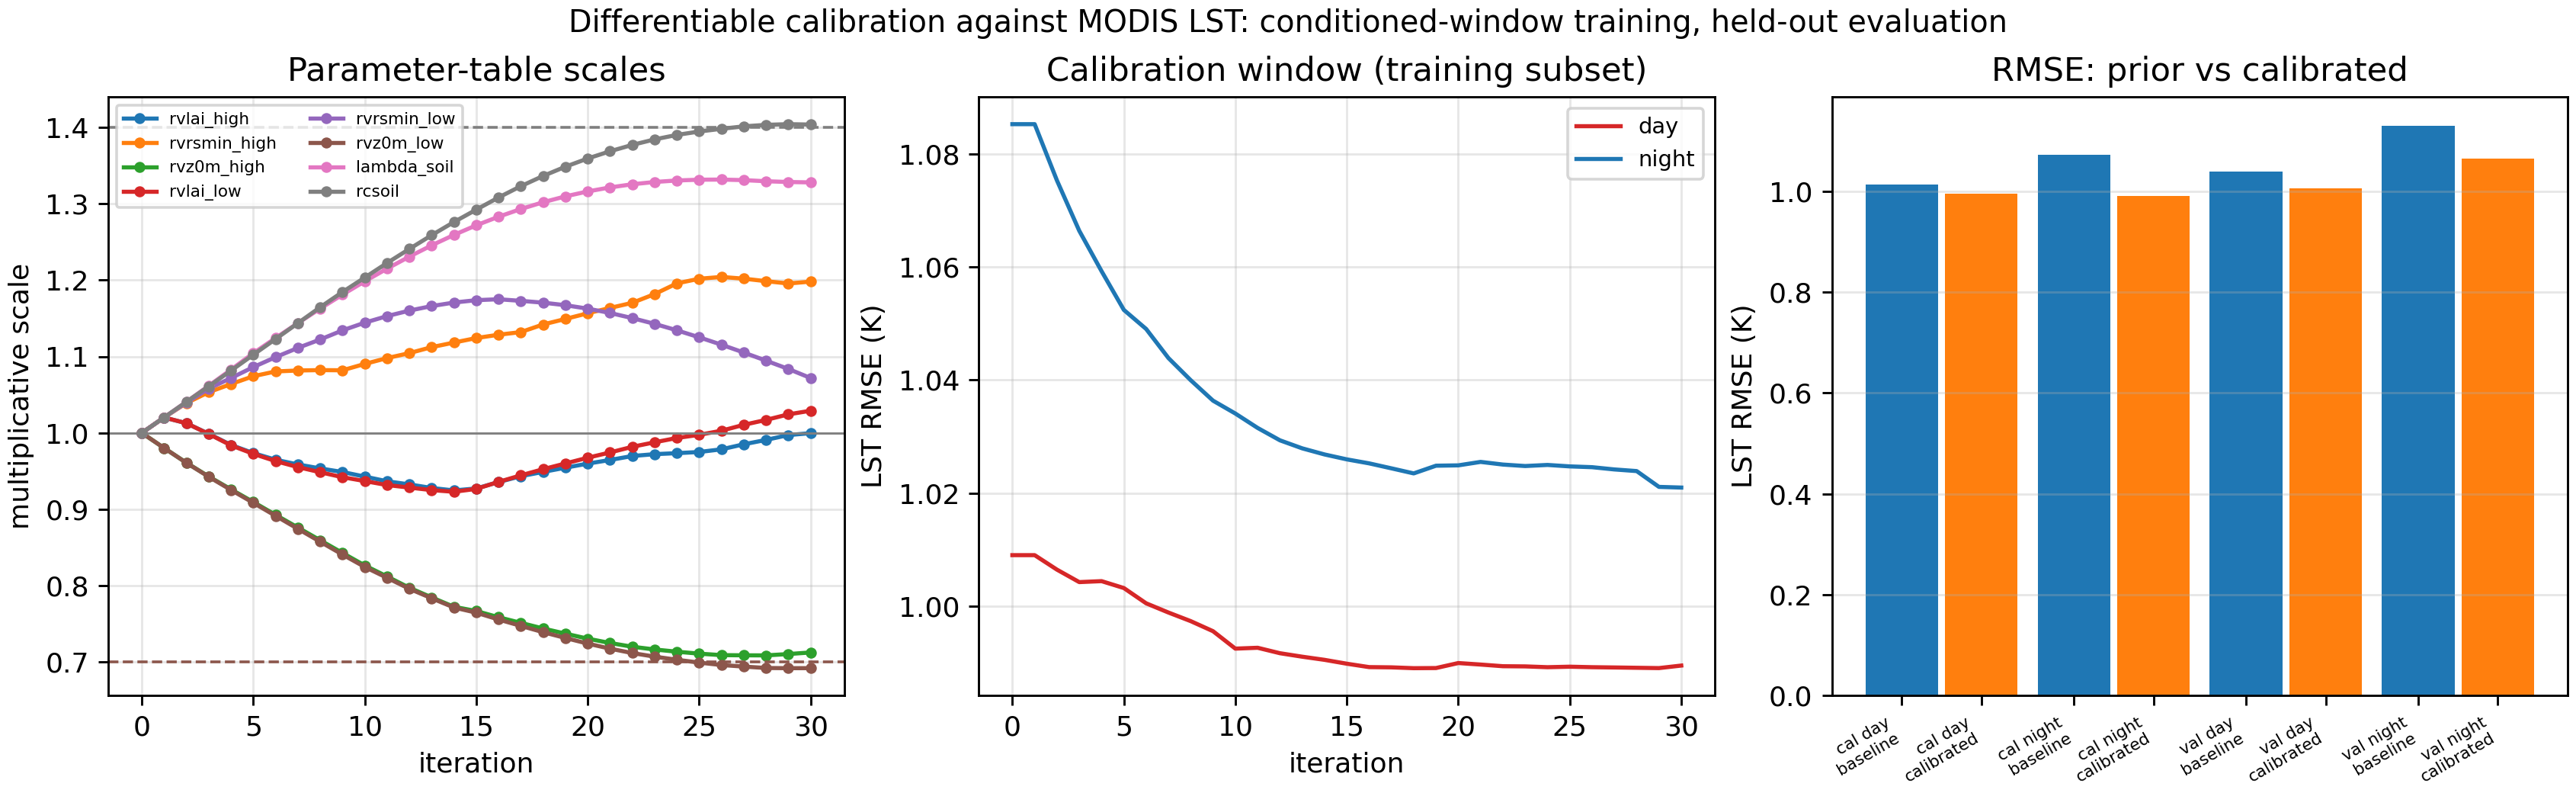
\includegraphics[width=\linewidth]{figures/modis_calibration_twin.png}
\caption{Observing-system simulation experiment with the real MODIS operator,
overpass times, and QC masks (1~K observation noise on the training subset).
Left: Adam trajectories of the eight table scales; dashed lines mark the
imposed truth values, and the two collinear unperturbed controls visibly
drift to compensating values. Centre: LST RMSE over the training subset,
converging to the noise floor. Right: prior-versus-calibrated RMSE in the
calibration and held-out windows.}
\label{fig:modis-calibration-twin}
\end{figure}

\begin{figure}[t]
\centering
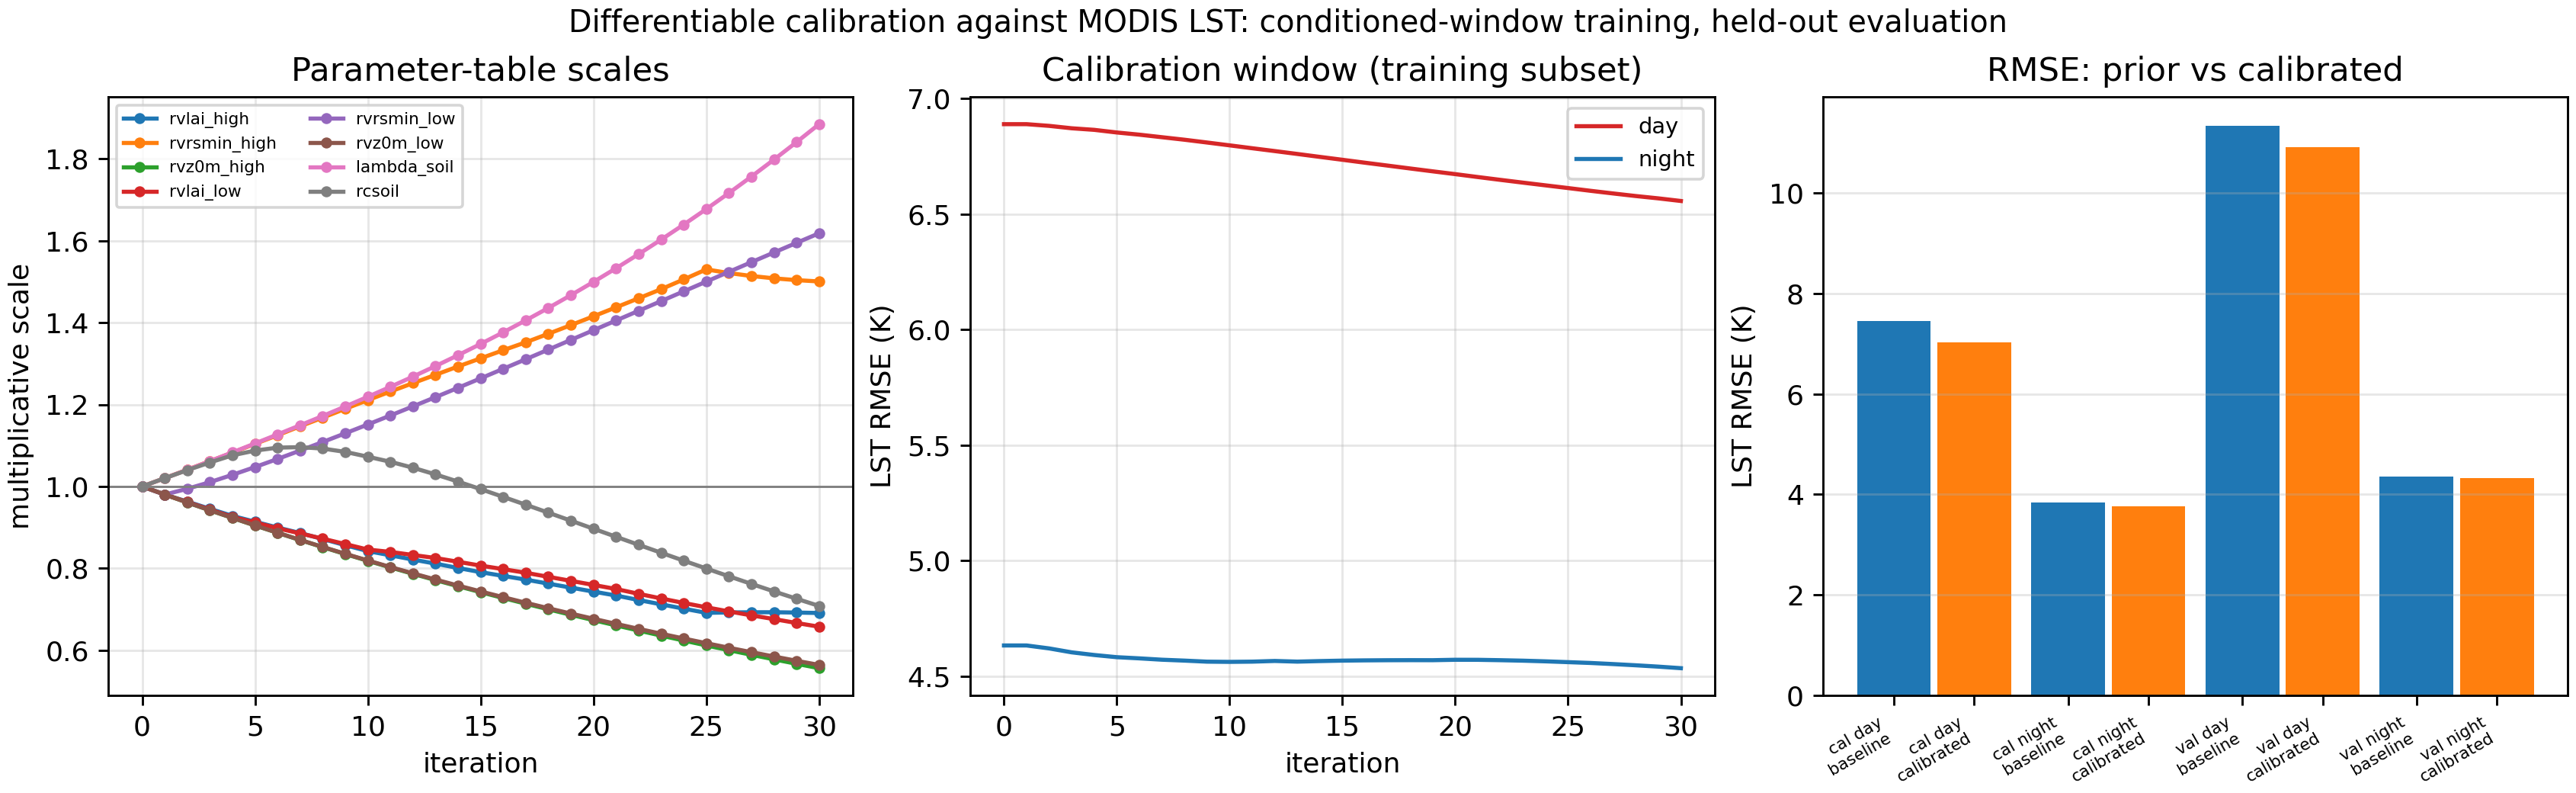
\includegraphics[width=\linewidth]{figures/modis_calibration_heldout.png}
\caption{Differentiable calibration against real MODIS Terra LST with an
identifiability-guided seasonal split (extended control vector). Left:
trajectories of the eight table scales; the roughness scales migrate toward
the lower admissible bound while compensating the structural daytime cold
bias. Centre: area-weighted LST RMSE over the training subset in the
autumn--winter calibration window. Right: full-domain prior-versus-calibrated
RMSE in the calibration and the held-out spring--summer windows, day and
night passes.}
\label{fig:modis-calibration}
\end{figure}

\subsection{Pseudo-forcing attribution}
\label{sec:structural-attribution}

The control vector of the final experiment is pseudo-forcing: eight additive
air-temperature offsets, one per local-time 3-hour bin, plus multiplicative
wind and shortwave scales (ten controls). A one-day finite-difference probe
already locates the leverage: the Terra day-overpass bin (09:00--12:00 local)
and the shortwave scale dominate ($|\Delta\mathcal{L}| \approx 4.1$ and
$7.1$ per $+0.5$~K and $+10\%$), the two nocturnal bins respond with
opposite sign (warming them degrades the night pass), and the early-morning
bins are nearly inert. Over 40 Adam iterations the calibration-window day
bias is largely removed ($-5.48$ to $-1.44$~K; RMSE $7.45$ to $5.11$~K) at
the optimal profile afternoon $+4.8$~K, evening $-3.1$~K, with the
shortwave scale unmoved at $1.0$ and the wind scale settling at $0.72$: the
radiative correction is redundant once the air-temperature profile is free
to move. The profile states what the offline configuration
lacks: a near-surface air-temperature diurnal amplitude about $8.1$~K
peak-to-peak larger than the reanalysis delivers, or an equivalent radiative
gain. Evaluated in the held-out spring--summer window under the same
anchored-day protocol, the corrections retain most of their effect (day
bias $-8.28$ to $-3.97$~K; day RMSE $11.34$ to $8.59$~K, night RMSE $4.35$
to $3.66$~K), so the diagnosed profile is seasonally robust
(Fig.~\ref{fig:modis-attribution}). It is not,
however, a parameterization: it is a ten-control additive adjustment of one
year's forcing fitted to one sensor, with no process form that could enter
the model physics or transfer to another forcing set. The diagnostic value
of the experiment lies in the shape of the required correction, not in the
number.

\subsection{Per-channel forcing sensitivity of daytime LST}
\label{sec:forcing-sensitivity}

The pseudo-forcing experiment of Sect.~\ref{sec:structural-attribution}
assigns leverage to air temperature and shortwave among ten controls. A
complementary single-channel check quantifies how strongly each forcing
channel of Eq.~(\ref{eq:model-forcing}) drives daytime land surface
temperature on its own. For each channel in turn, a single physically
meaningful perturbation is applied and the resulting change in domain-mean
day-pass LST is measured over a strong-insolation summer day (day of year
181) from the common spun-up restart. Because the perturbations have
different natural units and amplitudes, the comparison is made on a
normalized basis: the LST response per one-percent relative change of the
channel about its summer domain-mean value. Table~\ref{tab:forcing-sensitivity}
gives the result. The exchange air temperature dominates by an order of
magnitude over every other channel, about five times the next strongest
(downward longwave) and thirty times the shortwave, while humidity,
precipitation, and surface pressure are weak. This ordering is why the
closure of Sect.~\ref{sec:structural-slab} acts on the exchange air
temperature: it is the channel through which the diagnosed daytime deficit
is transmitted most strongly, and the radiative part of the deficit is
energetically equivalent to a correction of that same amplitude.

\begin{table}[t]
\caption{Single-channel forcing sensitivity of domain-mean day-pass LST
(day of year 181, spun-up restart, all 97{,}709 columns). For each forcing
channel a single perturbation is applied and the change in domain-mean day
LST is measured. The final column normalizes by the perturbation size as a
percentage of the channel's summer domain-mean value, making the channels
comparable.}
\label{tab:forcing-sensitivity}
\centering
\small
\begin{tabular}{llrr}
\hline
Channel & Perturbation & LST shift (K) & Sensitivity (K per 1\,\%) \\
\hline
Air temperature & $+1$~K & $+0.293$ & $+0.863$ \\
Downward longwave & $+10$~W\,m$^{-2}$ & $+0.457$ & $+0.160$ \\
Surface pressure & $\times 1.01$ & $+0.054$ & $+0.054$ \\
Wind speed & $\times 1.10$ & $+0.508$ & $+0.051$ \\
Specific humidity & $\times 1.10$ & $+0.390$ & $+0.039$ \\
Downward shortwave & $\times 1.10$ & $+0.268$ & $+0.027$ \\
Precipitation & $\times 2.0$ & $-0.142$ & $-0.001$ \\
\hline
\end{tabular}
\end{table}

\subsection{Timescale-asymmetry sweep and the state-space stability domain}
\label{sec:asym-sweep}

Before the two relaxation times of Sect.~\ref{sec:structural-slab} were
trained, a forward-only grid sweep with $\lambda_s = 0.05$ held fixed
mapped the response surface over $\tau_{day} \in \{3,5,10\}$~h and
$\tau_{night} \in \{1,2,3,5\}$~h under the anchored-day protocol. Every
statistically stable asymmetric combination improves on the tied closure in
both windows; the day-pass improvement grows monotonically as $\tau_{day}$
decreases, and the grid optimum ($\tau_{day} = 3$~h, $\tau_{night} =
2$--$3$~h) sits on the edge of the $\tau_{day}$ range, which motivated the
gradient calibration of Sect.~\ref{sec:structural-slab} over further grid
refinement. The sweep also delivered the first stability information:
$\tau_{night} = 1$~h is stable throughout the autumn--winter calibration
window yet destabilizes every held-out spring--summer integration
(day-pass biases of $10^{5}$--$10^{8}$~K). Statistical screening alone,
however, is not a sufficient acceptance test, and the unconstrained
training endpoint $(2.47, 2.36)$~h exposed why: it verifies on the
calibration window and on every held-out day pass, yet its held-out
integration of 11~May (day~131) diverges. We therefore re-verified the grid
in state space with a
step-level diagnostic that repeats the anchored-day protocol and records
the anomaly $\Delta T$ itself for every physics step and every column,
rather than view-time samples under quality control. The diagnostic is
bitwise-reproducible across two GPU architectures (A100 and RTX A6000), so
what follows is deterministic model dynamics, not hardware numerics. On
day~131 the failure is localized (Table~\ref{tab:asym-statespace}): 18
columns in two Tibetan-Plateau clusters (30--31$^\circ$N,
84--86$^\circ$E and 37--38$^\circ$N, 87--88$^\circ$E)
carry an intrinsic two-step ($\sim$1~h) limit cycle in the grid-mean
sensible heat flux $H$ (amplitude about $-100$ to $+150$~W~m$^{-2}$ at
vanishing anomaly): the offline exchange flips between stability regimes
through the dawn transition. The closure couples into this cycle through
its quasi-steady target $-\lambda_s H$. For the unconstrained endpoint, the
fatal columns respond at the dawn transition of the forecast day (steps
48--51, local 05:42--07:13), where the flux swings between about $-120$
and $+470$~W~m$^{-2}$ over consecutive steps; the anomaly passes 6~K by
step 55 and $10^{4}$~K by step 67, and the first non-finite state appears
at step 56, after which growth is superexponential. The domain is a
resonance structure, not a monotone boundary: ($\tau_{\mathrm{day}} = 4$~h,
$\tau_{\mathrm{night}} = 3$~h) diverges on day~131 while ($\tau_{\mathrm{day}}
= 5$~h, $\tau_{\mathrm{night}} = 3$~h) peaks at 54~K and
($\tau_{\mathrm{day}} = 4$~h, $\tau_{\mathrm{night}} = 4$~h) at
$2.5\times10^{2}$~K, so no axis-aligned interpolation of the statistical
sweep could have located it.

The most consequential property of this failure is that the
observation-space statistics cannot see it. The window aggregates of the
sweep remain clean at divergent grid points, $(3, 2)$, whose
day-131 state-space maximum is $9.4\times10^{20}$~K, and $(10, 2)$, which
exceeds $10^{3}$~K on day~341, because the strict MODIS quality control
removes exactly the divergent columns from the sampled statistics. A
verification protocol that scores only quality-controlled observations at
view times can therefore accept a configuration whose state space diverges;
monitoring the state itself is what separates the two. Applying the
step-level test to all 20 anchored evaluation days pins the
domain: $\tau_{\mathrm{night}} = 2$~h exceeds $10^{3}$~K on at least one
anchored day at $\tau_{\mathrm{day}} \in \{5, 8, 10\}$~h (days 121 and 341,
a few columns each) and stays finite but elevated at $\tau_{\mathrm{day}} =
6$~h (worst transient 150~K); $\tau_{\mathrm{day}} = 5$~h diverges on
day~121 at $\tau_{\mathrm{night}} \in \{2, 4, 5\}$~h while $(5, 3)$ stays
finite (worst 259~K); and $(6, 5)$ diverges on day~121. The combinations
$(6, 3)$, $(6, 4)$, and $\tau_{\mathrm{day}} \in \{8, 10\}$~h at
$\tau_{\mathrm{night}} \in \{3, 4, 5\}$~h pass all 20 days with no column
beyond 141~K, and the tied closure's worst transient is 49~K: the verified
set is not rectangular. These verified combinations form the training
domain of the constrained gradient calibration in
Sect.~\ref{sec:structural-slab}, whose optimum rests at their fastest
corner.

\begin{table}[t]
\caption{State-space verification of the closure grid on held-out day~131:
maximum $|\Delta T|$ (K) over all columns and all 96 anchored steps.
``Diverged'' marks non-finite states. The combinations adopted for training
also pass the same test on all 20 anchored evaluation days (worst
single-column transient 109~K at $(\tau_{\mathrm{day}}, \tau_{\mathrm{night}})
= (6, 3)$~h, decaying); $\tau_{\mathrm{night}} = 2$~h exceeds $10^{3}$~K on
day~341 at $\tau_{\mathrm{day}} \in \{5, 8, 10\}$~h and on day~121 at
$\tau_{\mathrm{day}} = 5$~h. The tied closure (10.1~h, 10.1~h) peaks at 34~K
on this day.}
\label{tab:asym-statespace}
\centering
\small
\begin{tabular}{lrrrrrr}
\hline
 & $\tau_{\rm day}=3$~h & $\tau_{\rm day}=4$~h & $\tau_{\rm day}=5$~h &
   $\tau_{\rm day}=6$~h & $\tau_{\rm day}=8$~h & $\tau_{\rm day}=10$~h \\
\hline
$\tau_{\rm night}=2$~h & $9.4\times10^{20}$ & $3.7\times10^{2}$ &
  $1.6\times10^{2}$ & 65 & 61 & 48 \\
$\tau_{\rm night}=3$~h & $9.8\times10^{7}$ & diverged &
  54 & 78 & 51 & 29 \\
$\tau_{\rm night}=4$~h & diverged & $2.5\times10^{2}$ & 48 & 60 & 42 & 39 \\
$\tau_{\rm night}=5$~h & diverged & $2.1\times10^{2}$ & 64 & 65 & 44 & 29 \\
\hline
\end{tabular}
\end{table}

